\documentclass[25pt, a0paper, portrait]{tikzposter}
\geometry{paperwidth=34in,paperheight=36in}

\title{Simulating Missile Trajectory with DEs}
\author{Colin Tierney}
\date{\today}
\institute{Modeling and Simulation Final}
\usebackgroundstyle{Default}

\usepackage{blindtext}


\usetheme{Default}
\definebackgroundstyle{Default}{
\draw[inner sep=0pt, line width=0pt, color=white, fill=white]
(bottomleft) rectangle (topright);}


\begin{document}

\maketitle
\node[anchor=west, xshift=-2cm] at (TP@title.west) {
\includegraphics[width=10cm]{images/mc-logo}};
\node[anchor=east, xshift=1cm, yshift=-.25cm] at (TP@title.east) {
\includegraphics[width=8cm]{images/qrcode}};


\begin{columns}
    \column{0.6}     
    \block{Introduction}
    {
        In a ballistic missile trajectory simulation, the system of DEs used to describe the ballistic 
        model is a highly complex system. In particular, the six-degree of freedom model used most 
        frequently, solves for the missile's components of acceleration, velocity, and position at discrete 
        time intervals. The usual approach for simulation is the 4th Order Runge Kutta method. This poster 
        will be diving into a different, and potentially more efficient algorithm, called the 
        Parker-Sochacki Method (PSM for short).
    }
    \column{0.4}
    \block{Assumptions}
    {           
        Variables used/Assumptions used in model
    }
\end{columns}


\begin{columns}
    \column{0.4}
    \block{Problem Identification}
    {
        Here, \blindtext
    }   
    \column{0.6}
    \block{Cauchy Product Derivation}
    {
        
    }
\end{columns}


\begin{columns}
    \column{0.5}
    \block{Model Verification}
    {
        \begin{tikzfigure}
            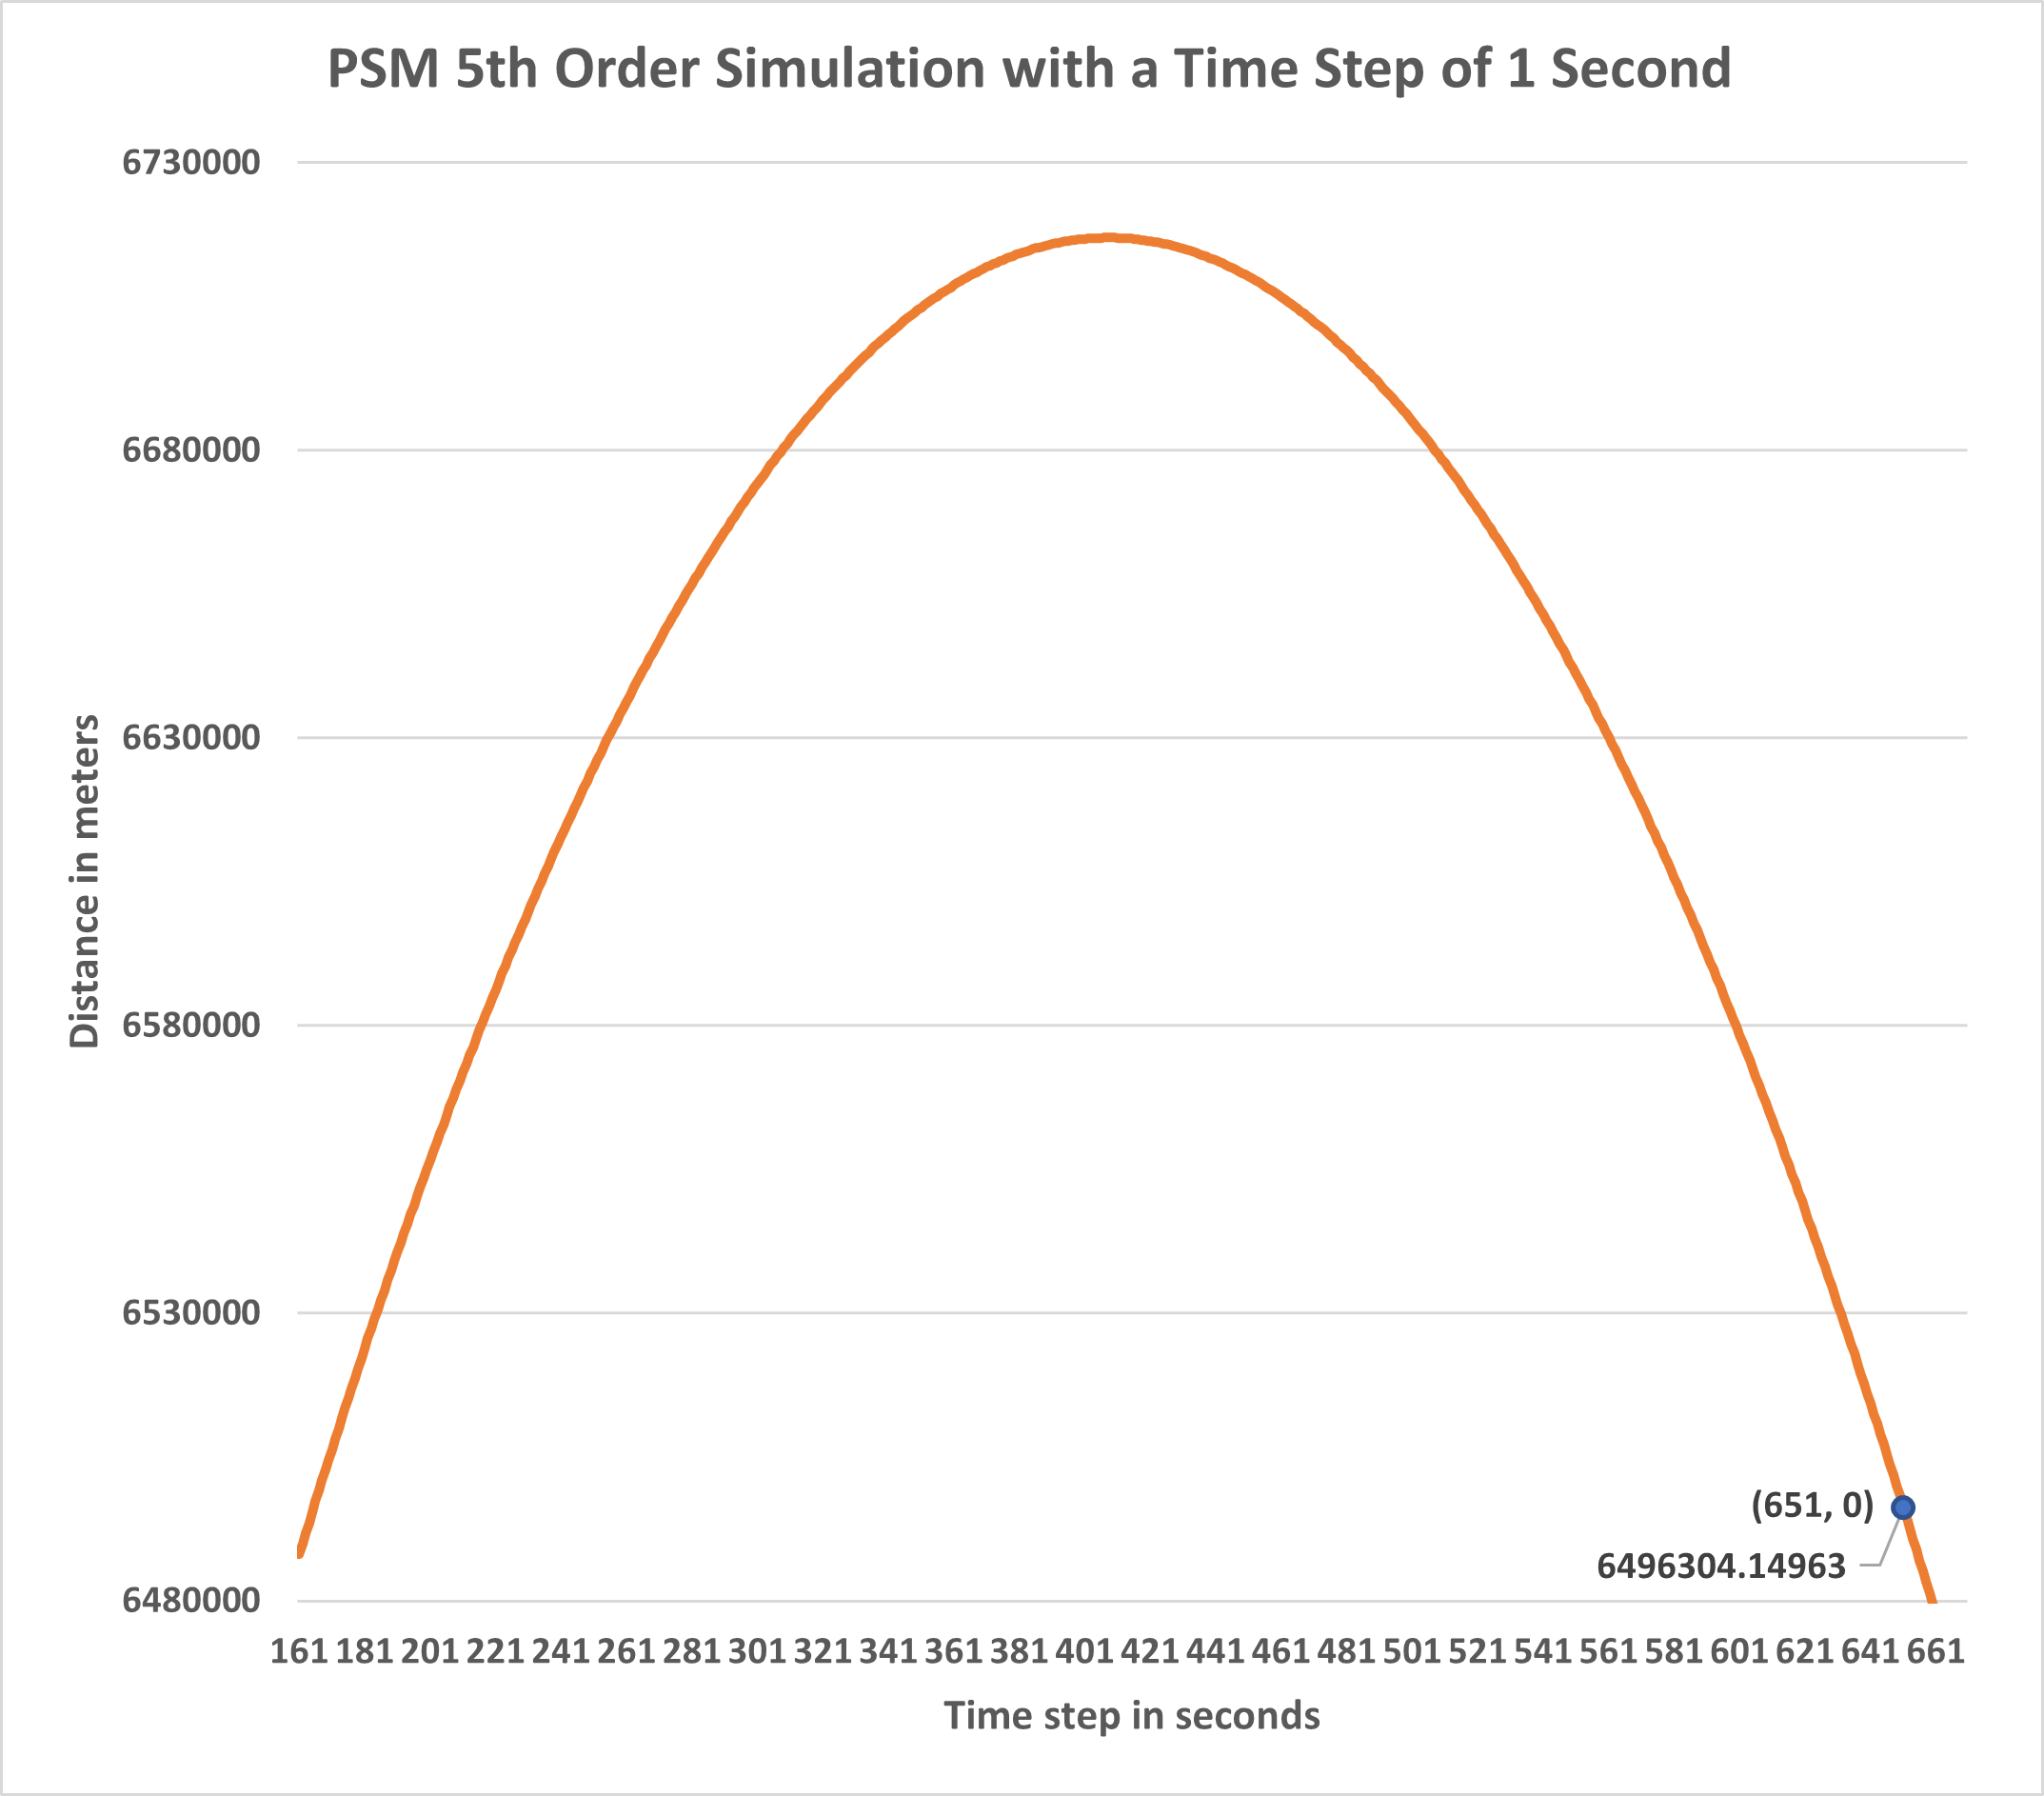
\includegraphics[width=0.2\textwidth]{images/PSM5 TS1 Plot.png}
        \end{tikzfigure}
        Hello
    }
    \column{0.5}
    \block{Figures}
    {
        \blindtext
    }
    \block{Conclusion}
    {
        conclusion stuff
    }
\end{columns}
\block{References}
{
    \blindtext
}


\end{document}